
\subsubsection{Qualification}

\begin{figure*}[!htb]
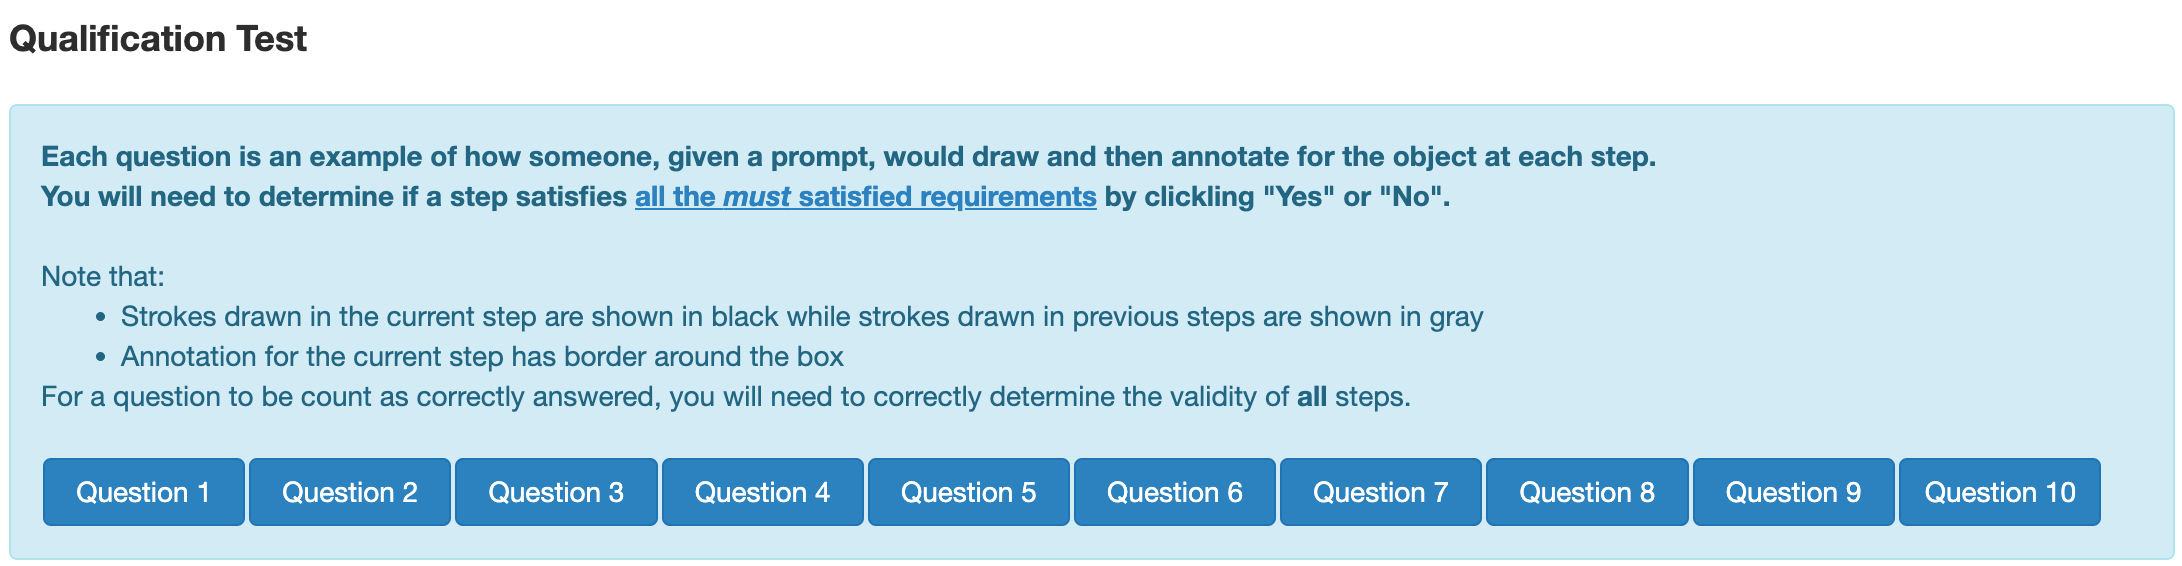
\includegraphics[width=\linewidth]{data_collection/v1_qual_header.png}  
\caption{Navigation bar in the qualification test.}
\label{v1.qualification.nav}
\end{figure*}

\begin{figure*}[!htb]
\begin{subfigure}{\textwidth}
\centering
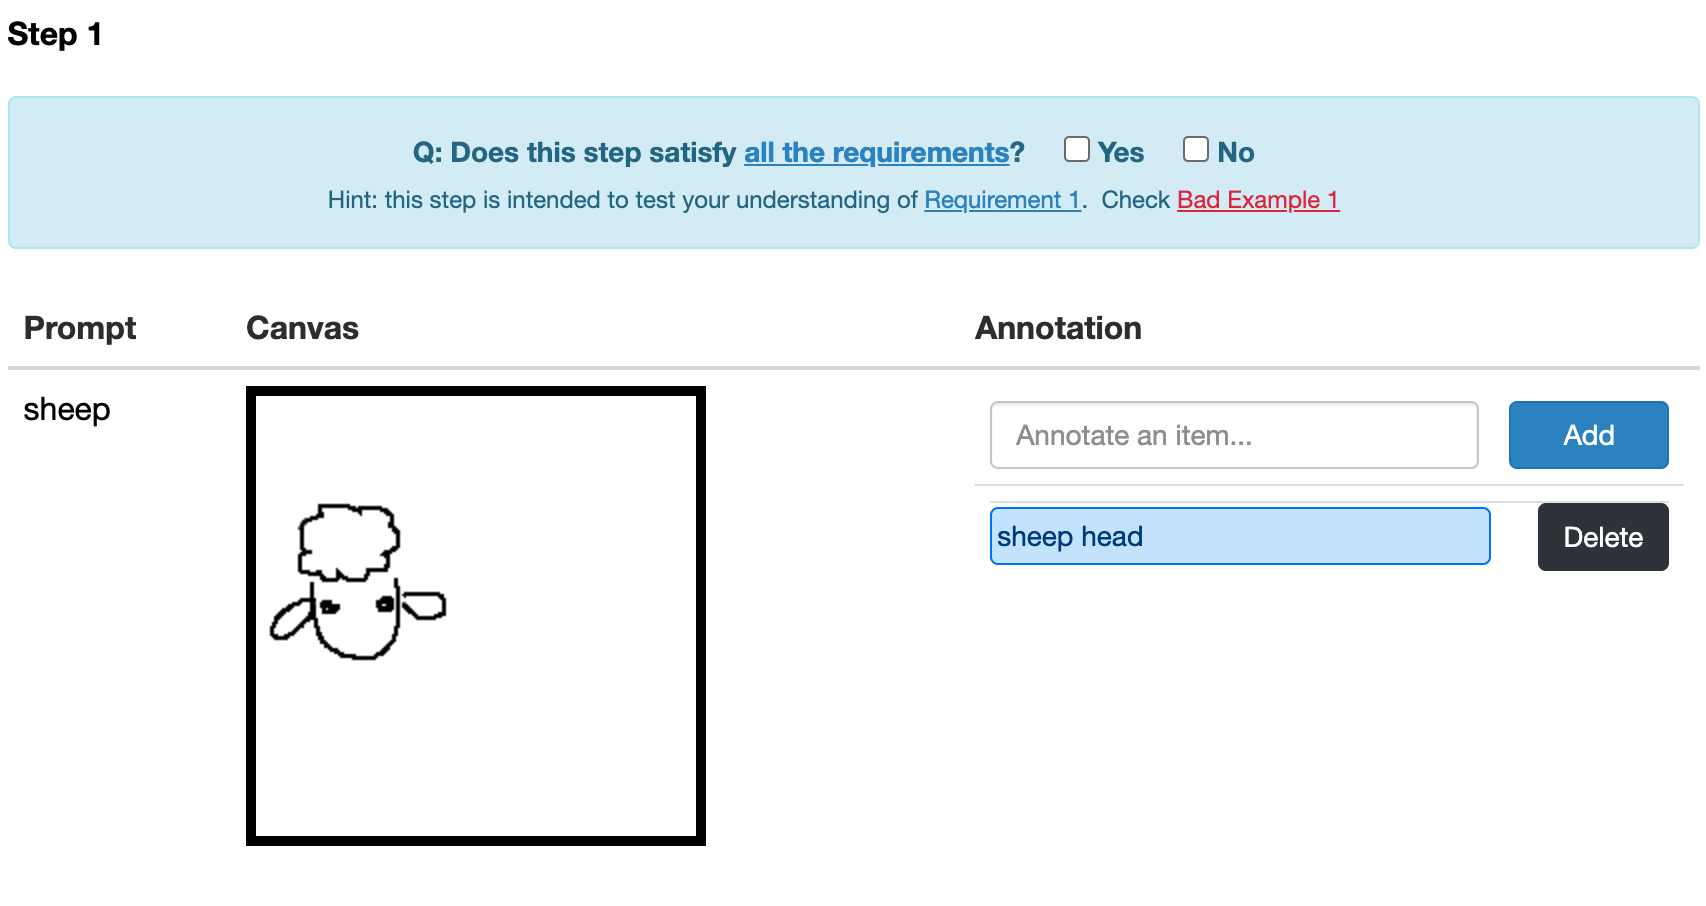
\includegraphics[width=.8\linewidth]{data_collection/v1_qual_q9_1.png}  
\end{subfigure}
\newline
\begin{subfigure}{\textwidth}
\centering
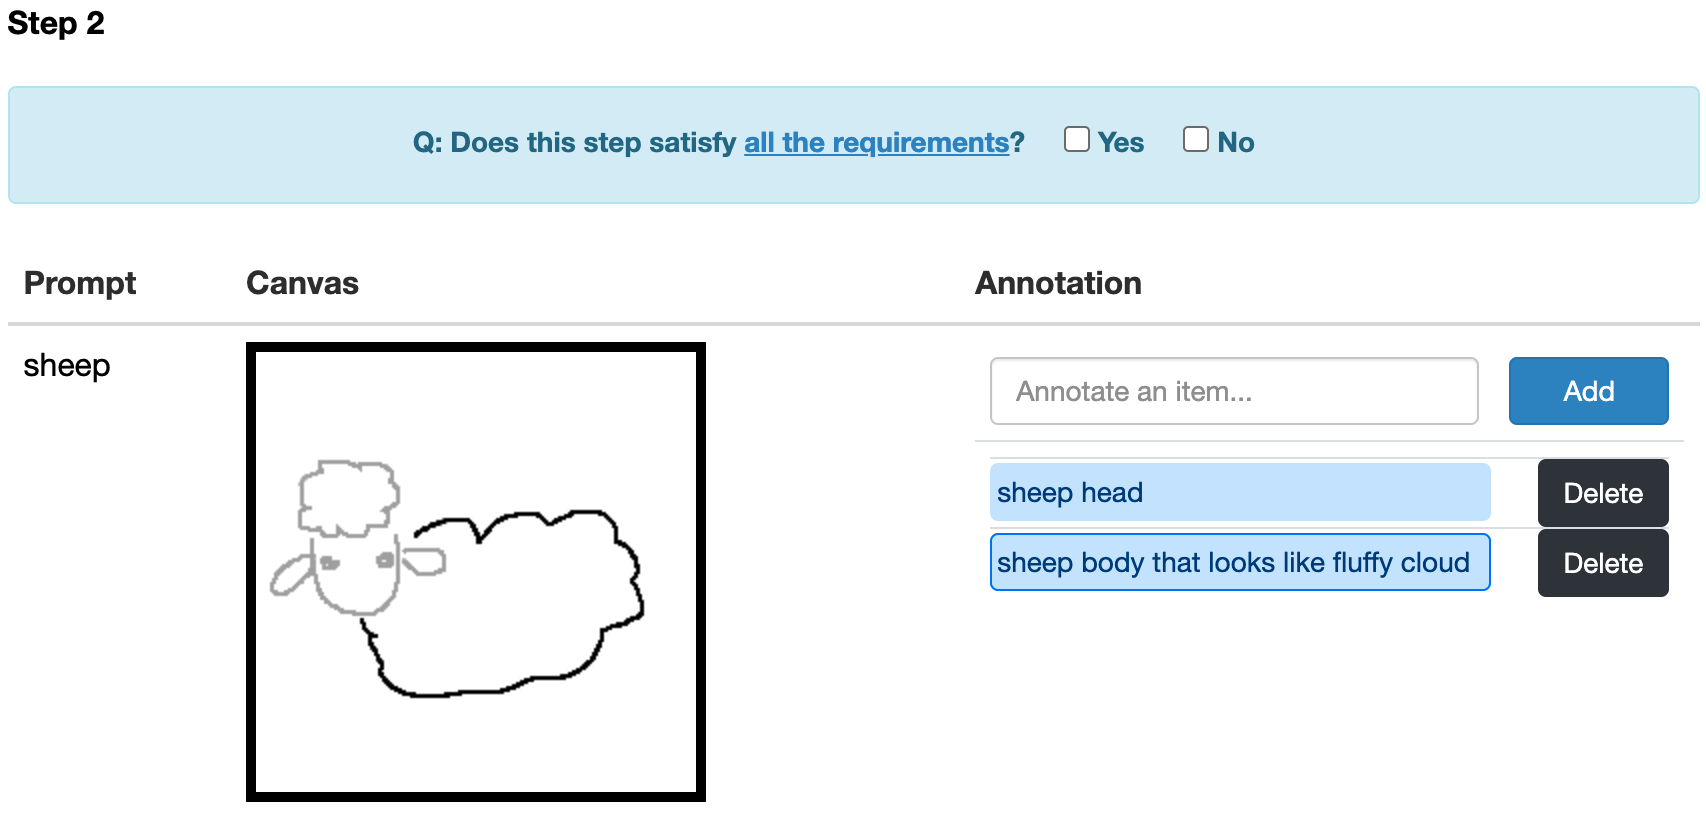
\includegraphics[width=.8\linewidth]{data_collection/v1_qual_q9_2.png}  
\end{subfigure}
\caption{An example of the questions in the qualification test.}
\label{v1.qualification.q9}
\end{figure*}

We set up a qualification test on AMT to (1) train turkers to have better understanding of the task and (2) to select turkers who can provide annotations that satisfy all the requirements. 
Similar to the process of writing the requirements, we went through several rounds of testing with students in the lab to come up with a set of questions that correspond well with the requirements. 
The qualification test starts with the same instruction and requirements in the final HIT, thus allowing turkers to familiarize themselves with the requirements and ask clarification questions before completing the actual annotation task. 
The test leads with a navigation bar (Figure \ref{v1.qualification.nav}) to make it convenient for turkers to switch between questions; originally, we displayed all questions on one page, but some found it time-consuming to scroll from the later questions back up to the instructions, so we decided to display one question at a time. 
We show one question from the final qualification in Figure \ref{v1.qualification.q9}. 
Each question is a mock-up of the main task interface, and turkers need to determine whether every step satisfies all the requirements.
We also include hints on which requirement the question is testing to encourage turkers to revisit the requirements and form better understanding of the task.  
To see the full test, refer to: \url{https://erinzhang1998.github.io/portfolio/amazon_qual}.

% [Figure x5: final qualification test]
%  At first, we asked the annotators to select which steps of the annotations satisfy the requirements (Figure x6.a); in order to use repetition to ensure deep understanding of the requirements, we changed to asking a yes/no question for every step, as shown in Figure x6.b.  
